\documentclass[compress]{beamer}%
\usepackage[utf8]{inputenc}
\usetheme{Warsaw}

% \usepackage

\title{Initiation aux frameworks : \emph{Spring}}
\subtitle{Spring et les concepts de l'inversion de Contrôle}

\author{Thomas Duchatelle (duchatelle.thomas@gmail.com)}
\institute{Capgemini, pour Yves Rocher}

\setbeamertemplate{navigation symbols}{} 
\useoutertheme{infolines}
\setbeamertemplate{footline}
{%
  \leavevmode%
  \hbox{\begin{beamercolorbox}[wd=.5\paperwidth,ht=2.5ex,dp=1.125ex,leftskip=.3cm plus1fill,rightskip=.3cm]{author in head/foot}%
    \usebeamerfont{author in head/foot}\insertshortauthor
  \end{beamercolorbox}%
  \begin{beamercolorbox}[wd=.41\paperwidth,ht=2.5ex,dp=1.125ex,leftskip=.3cm,rightskip=.3cm plus1fil]{title in head/foot}%
    \usebeamerfont{title in head/foot}\insertshorttitle 
  \end{beamercolorbox}%
  \begin{beamercolorbox}[wd=.09\paperwidth,ht=2.5ex,dp=1.125ex,leftskip=.3cm plus1fill,rightskip=.3cm]{author in head/foot}%
    \usebeamerfont{author in head/foot}\insertframenumber/\inserttotalframenumber
  \end{beamercolorbox}}%
  \vskip0pt%
}

\AtBeginSection[]{
  \begin{frame}{Sommaire}
  \small \tableofcontents[currentsection, hideothersubsections]
  \end{frame} 
}

\definecolor{fontcolor}{rgb}{0.92,0.92,0.99}
\usepackage{listings}
\lstset{language=Java, numbers=left, tabsize=2, frame=single, breaklines=true,  numberstyle=\tiny\ttfamily,basicstyle=\small, framexleftmargin=5mm, backgroundcolor=\color{fontcolor}, xleftmargin=5mm, basicstyle=\tiny }

\graphicspath{images}

\begin{document}


% Pages de présentations...
\frame{\titlepage}
  
\section*{Plan}
\frame{\tableofcontents[hideallsubsections]}
	
%%%%%%%%%%%%%%%%%%%%%%%%%%%%%%%%%%%%%%%%%
%% SOA
\section{Séparation des préoccupations}

\subsection{Définition}

\begin{frame}{Séparation des préoccupations}
%	\framesubtitle{SoC}
	
	\begin{block}{SoC : Separation of Concerns}
	Pris isolément, chaque problème est plus facile à traiter.
	\end{block}

	\pause
	Découpage de l'application pour isoler les problématiques :
	\begin{itemize}
	\item persistance
	\item services métier
	\item présentation (IHM Web)
	\item appel webservice
	\item ...
	\end{itemize}
	
	\pause
	\begin{block}{Beans}
	Pour chaque nature de problématique : conception de "composants spécialisés", de \emph{briques applicatives}.
	\end{block}
\end{frame}

\subsection{Cas concret}

\begin{frame}{Cas concret}
	\framesubtitle{Embauche d'un nouvel employé}
	
	\begin{exampleblock}{Nouvelle embauche}
	Intégration dans le SI d'un nouvel employé : création de son matricule, email et insertion dans le système des ressources humaines.
	\end{exampleblock}
	
	\pause
	Processus métier pour l'embauche d'un nouveau client :
	\begin{enumerate}[<+->]
		\item un administrateur renseigne le nom, prénom et intitulé du poste du nouvel employé
		\item le système génère le matricule de l'employé : identifiant unique
		\item le système génère l'email de l'employé : à partir de son nom et prénom, unique aussi
		\item toutes ces données sont conservées dans le Référentiel Employés
		\item le système informe l'application des Ressources Humaines de la création de nouvel employé
	\end{enumerate}	
	
\end{frame}

\begin{frame}{Méga script !}
	\framesubtitle{Un script PHP suffit}
	
	\begin{itemize}[<+->]
	\item Un tel processus pourrait être écrit en un seul script PHP...\\
	\item Mais :
	\begin{itemize}[<+->]
	\item difficulté d'écrire le script
	\item longueur et lisibilité du script ?
	\item tests de tous les cas
	\item gestion des cas d'erreurs
	\end{itemize}
	\end{itemize}
	
\end{frame}

\begin{frame}{Séparation des préoccupations}
	\framesubtitle{Division de la problématique en petites sous problématique}
	
	Proposition de découpage :
	\pause
	\begin{itemize}[<+->]
	\item \emph{IHM} (couche de présentation) : propose une interface intuitive à l'administrateur afin de récolter les données
	\item \emph{Gestionnaire des Employés} (objet métier) : détient les règles et le processus de création d'un employé
	\item \emph{Générateur de matricules} (objet métier) : détient les règles de génération d'un identifiant unique
	\item \emph{Générateur d'email} (objet métier) : génère un email à partir du nom et prénom.
	\item \emph{DAO Employés} (objet d'accès aux données) : persiste l'employé et détermine si un email est disponible
	\item \emph{Connecteur Webservice Ressources Humaines} (objet métier) : gère la connexion avec le webservice de l'application des RH.
	\end{itemize}
	
\end{frame}

\begin{frame}
	\frametitle{Architecture de l'exemple}

	%% TODO Corriger la faute dans l'image : matriculeS (au pluriel)
	\begin{center}	
	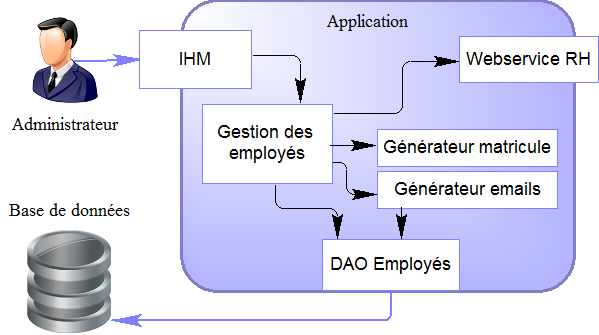
\includegraphics[width=\textwidth]{images/spring_usecase.png}
	\end{center}
\end{frame}



\begin{frame}	
	\begin{center}	
	\Large
	Comment gérer efficacement toutes ces briques applicatives ?
	\end{center}
\end{frame}
	

\section{Inversion de contrôle}

\subsection{Définitions}

\begin{frame}{Inversion de Contrôle}
	\framesubtitle{Association de 3 grands patterns}
	
	\begin{columns}
		\begin{column}{0.5\textwidth}
			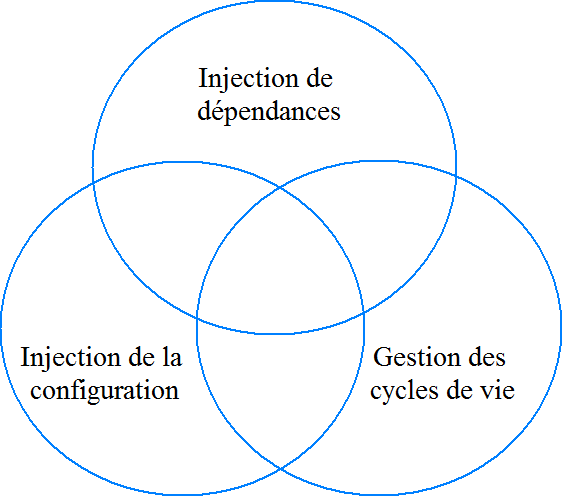
\includegraphics[width=\textwidth]{images/spring_ioc.png}
		\end{column}
		\begin{column}{0.5\textwidth}
			Les 3 grands patterns :
			\begin{itemize}
			\item \textbf{Injection de dépendances}	
			\item \textbf{Injection de la configuration}
			\item \textbf{Gestion des cycles de vie}
			\end{itemize}
		\end{column}
	\end{columns}

\end{frame}

\begin{frame}{Conteneur}
	\framesubtitle{Différents types de conteneurs}

	\begin{block}{Conteneur}
		Infrastructure fournissant l'inversion de contrôle : gestion du cycle de vie, injection des dépendances, injection de la configuration.
	\end{block}

	\pause
	Il en existe de 2 types :
	\begin{itemize}
		\item \textbf{Conteneur lourd} : intégré à une applicatition à par entière, un serveur d'applications (Websphère, Tomcat, JBoss, \dots)
		\item \textbf{Conteneur léger} : le conteneur n'est qu'une librairie embarquée dans l'application, moins intrusive et plus flexible (\emph{Spring}, Guice)
	\end{itemize}
\end{frame}

\subsection{Cycle de vie}
% c'est Spring qui décide quand créer un objet, et quand le détruire.

\begin{frame}[fragile]{Gestion du cycle de vie}

	\begin{block}{Vie d'un objet}
	Un objet est instancié (créé) à l'aide du mot clef \texttt{new} et est détruit par le \emph{garbage collector} lorsqu'il n'est plus référencé.
	\end{block}

	\begin{lstlisting}
// Intanciation d'un nouvel employe
Employee employee = new Employee();
	\end{lstlisting}


	\pause
	\begin{block}{Cycle de vie}
	Gérer le cycle de vie d'un objet consiste à le créer lorsqu'il est utile, et le déréférencer lorsqu'on en a plus besoin.
	\end{block}

\end{frame}

\begin{frame}

	\begin{block}{Portée}
		La portée défini la validité d'une instance en fonction du contexte. Autrement dit, savoir quand une instance doit être réutilisée, ou quand une nouvelle instance doit être créée.
	\end{block}

	\pause
	Portées possibles d'un bean :
	\begin{itemize}[<+->]
		\item \textbf{singleton} : une seule instance est créée pour l'ensemble de l'application, en général au lancement de l'application. Elle n'est détruite qu'à l'arrêt de l'application
		\item \textbf{prototype} : une instance est créée à chaque demande, elle est déréférencée dès que possible
		\item "pool" : un nombre fini d'instances sont créées. Elles sont fournies aux objets qui en ont besoin, ces derniers les libérent lorsqu'ils sont détruits, ou qu'ils n'en ont plus besoin.
		\item \emph{session / request} : portées spécifiques à un contexte WEB
	\end{itemize}
	
\end{frame}

\begin{frame}[fragile]{Exemples de code}

	 Sans gestion du cycle de vie : 
	\begin{lstlisting}
// Instance de type singleton (2 solutions) :
EmployeeNumberGenerator generator1 = EmployeeNumberGenerator.getInstance();
EmployeeNumberGenerator generator2 = Factory.getEmployeeNumberGenerator();

// Instance de type prototype :
PayReport report = new PayReport();
	\end{lstlisting}

	\pause
	Avec gestion du cycle de vie
	\begin{lstlisting}
// Demande au context du conteneur une instance du type voulu
EmployeeNumberGenerator employeeNumberGenerator = applicationContext.getBean(EmployeeNumberGenerator.class);
	\end{lstlisting}

	\pause
	\begin{block}{Conteneur}
		Ce n'est plus le code qui détermine si l'objet est un singleton ou un prototype, mais la \textbf{configuration du conteneur}.
	\end{block}

\end{frame}


\subsection{Injection des dépendances}

\begin{frame}{Injection de dépendances}

	\begin{block}{Dépendance}
		Certaines briques applicatives utilisent d'autres briques pour fonctionner. Ces briques nécessaires au fonctionnement sont appelées \textbf{dépendances}.
	\end{block}

	\pause
	\begin{exampleblock}{Exemples}
		Le bean "\emph{générateur d'emails}" a 1 dépendance : \emph{DAO Employés}.

	\pause
		Le bean "\emph{gestion des employés}" a 4 dépendances :
		\begin{itemize}
			\item \emph{générateur de matricules}
			\item \emph{générateur d'emails}
			\item \emph{DAO Employés}
			\item \emph{Connecteur Webservice RH}
		\end{itemize}
	\end{exampleblock}

\end{frame}

\begin{frame}%[fragile]

	\begin{block}{Injecter une dépendance}
		\`A la création d'un bean, ses dépendances sont instanciées et lui sont affectées (injectées).
	\end{block}

	\pause
% 	\begin{lstlisting}
% public class EmailGenerator {
% 
%   private EmployeeDAO employeeDAO;
% 
%   public void uneMethode() {
%     // employeeDAO n'est PAS nul : il a ete injecte à la creation de l'EmailGenerator.
%     employeeDAO.emailExists("un@email.com");
%   }
% }
% 	\end{lstlisting}
	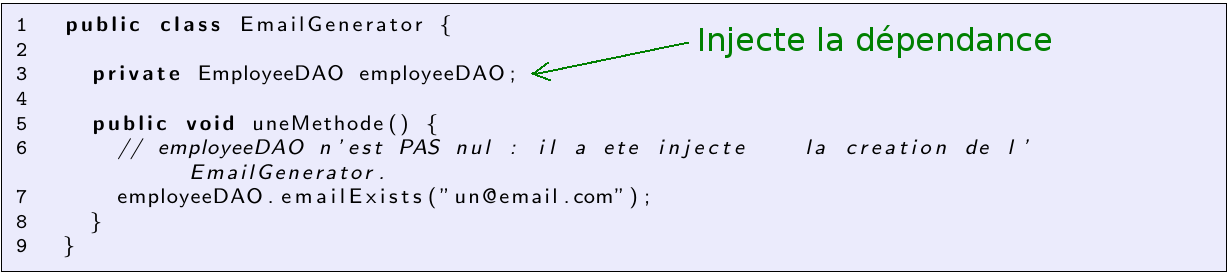
\includegraphics[width=\textwidth]{images/inject_code.png}


\end{frame}

\subsection{Gestion de la configuration}

\begin{frame}{Gestion de la configuration}
	\framesubtitle{... par injection !}

	\begin{block}{Injection de la configuration}
	La configuration est paramétrée de façon globale (fichiers properties, dictionnaire jndi, ...), et elle est distribuée à tous les beans qui en ont besoin.
	\end{block}
\end{frame}

\begin{frame}

	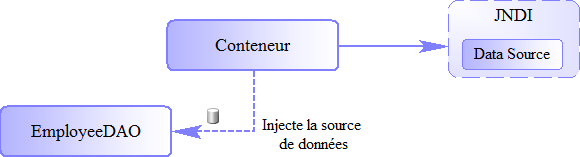
\includegraphics[width=\textwidth]{images/spring_datasource_with.png}

	\pause
	\begin{itemize}[<+->]
		\item \textbf{Couplage lâche} : \texttt{EmployeeDAO} n'a pas connaissance de la façon dont sont configurées les sources de données.
		\item \emph{Gestion des portée} : la source de données injectée peut dépendre d'un contexte (pays).
		\item \emph{Cohérence} : toute l'application, voire même \emph{les} applications, sont configurées de la même façon.
	\end{itemize}
\end{frame}

\subsection{Environnements multiples}

\begin{frame}{Environnements multiples}
	\framesubtitle{Différences d'environnements}

	\begin{center}
		Comment gérer les différences entre un environnement \emph{WEB}, et \emph{Batch} ?
	\end{center}

	\pause
	\begin{block}{Alternatives}
		En remplaçant, ou ajoutant, un fichier de configuration à l'initiation du contenaire, il est possible de chager l'implémentation d'un bean.
	\end{block}

\end{frame}

\begin{frame}

	\begin{exampleblock}{Configuration dans un contexte WEB et Batch}
		Dans un environnement WEB, les sources de données sont configurées dans un dictionnaire JNDI. Mais dans l'environnement Batch, elles sont configurées dans un fichier.
	\end{exampleblock}

	\pause
	\begin{itemize}
		\item Ajout d'une alternative : chargement de sources de données via un fichier.
	\end{itemize}


	\pause
	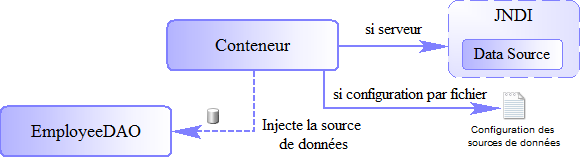
\includegraphics[width=\textwidth]{images/spring_datasource_with_full.png}
\end{frame}


%%%%%%%%%%%%%%%%%%%%%%%%%%%%%%%%%%%%%%%%
%% SPRING

\section{Spring}

\subsection{Définition}
% conteneur léger ? pas d'application, seulement un JAR
% opposition avec les EJB qui demandent un serveur d'applications (Websphère)

% Cartography "IoC et bien autres choses !"

\begin{frame}{Spring = Conteneur léger !}
	\framesubtitle{Définitions ...}

% 	\begin{description}
% 		\item[Conteneur] Infrastructure prenant en charge la création d'objets et leurs dépendances : mise en relation d'objets via des fichiers de configuration.
% 		\pause
% 		\item[Conteneur \emph{lourd}] : le conteneur prend la forme d'une application complète sur laquelle est intallé l'application cliente. Exemple : Websphere, Tomcat, JBoss, ...
% 		\pause
% 		\item [Conteneur \emph{léger}] : le conteneur n'est qu'une librairie embarquée dans l'application. Elle est initialisée programmatiquement.
% 	\end{description}
% 
% 	\pause
	\begin{block}{Spring}
		\textbf{Spring est un conteneur léger.}\par
		Il se présente comme un ensemble de librairies à embarquer dans l'application. Il founit l'\emph{inversion de contrôle} : gestion du cycle de vie, injection des dépendances, injection de la configuration.
	\end{block}

	\pause
	\begin{center}
		\large
		Mais pas que ...
	\end{center}
\end{frame}

\begin{frame}{Spring, la boite à outils du développeur JAVA}

	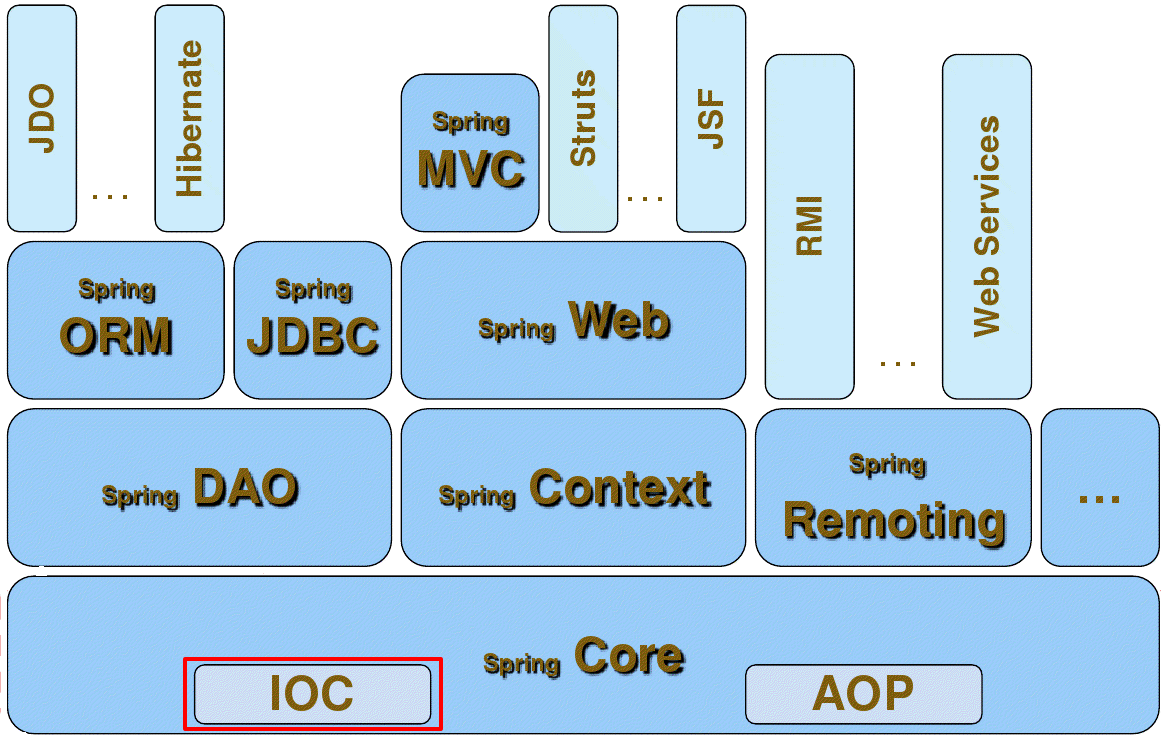
\includegraphics[width=\textwidth]{images/spring_cartography.png}

\end{frame}

\subsection{Configuration du contenaire}

% XML => déclaration de l'utilisation des annotations
% Création d'un contexte applicatif => uniquement en Java SE
\begin{frame}[fragile]{Configuration du contenaire}
	\framesubtitle{Instanciation de l'\emph{application context}}

	\begin{block}{\texttt{ApplicationContext}}
		Le contenaire de \emph{Spring} s'appelle \texttt{ApplicationContext}. Il est créé à partir d'un fichier de configuration XML.
	\end{block}

	\pause
	\begin{lstlisting}
ApplicationContext context = new ClassPathXmlApplicationContext("context.xml");
	\end{lstlisting}

\end{frame}


\begin{frame}[containsverbatim]{Configuration du contenaire}
	\framesubtitle{Contenu du fichier XML}

	Fichier \texttt{context.xml} : 
	\lstset{language=XML}
	\begin{lstlisting}
<?xml version="1.0" encoding="UTF-8"?>
<beans xmlns="http://www.springframework.org/schema/beans"
	xmlns:xsi="http://www.w3.org/2001/XMLSchema-instance" xmlns:context="http://www.springframework.org/schema/context"
	xsi:schemaLocation="http://www.springframework.org/schema/beans http://www.springframework.org/schema/beans/spring-beans.xsd
		http://www.springframework.org/schema/context http://www.springframework.org/schema/context/spring-context-3.1.xsd">

	<!-- Active les annotations pour le package donne -->
	<context:annotation-config />
	<context:component-scan base-package="net.yvesrocher.tutorial.employees" />

	<!-- Lecture des fichiers de proprietes (tous les fichiers dans config) -->
	<context:property-placeholder location="classpath:config/*.properties"/>
	
</beans>
	\end{lstlisting}
	\lstset{language=JAVA}

\end{frame}


\subsection{Annotations Spring}
% Déclaration d'un Bean
\begin{frame}[fragile]{Déclarer un bean}

	\begin{block}{\texttt{$@$Named}}
		Les beans sont déclarés par l'annotation \texttt{$@$Named} placé au dessus de la classe.
	\end{block}

	\pause
	\begin{lstlisting}
@Named
public class EmployeeManager {
}
	\end{lstlisting}

\end{frame}

\begin{frame}[fragile]{Limiter la portée d'un bean}

	\begin{block}{\texttt{$@$Scope}}
		L'annotation \texttt{$@$Scope} défini la portée du bean. La portée par défaut avec \emph{Spring} est \texttt{singleton}
	\end{block}

	\pause
	\begin{lstlisting}
@Named
@Scope("singleton")
public class EmployeeManager {
}
	\end{lstlisting}

	\pause
	Rappels :
	\begin{description}
		\item[Singleton] : une seule instance est créée pour toute l'application.
		\item[Prototype] : une instance est créée à chaque demande
	\end{description}


\end{frame}

% Injection d'une dépendance
\begin{frame}[fragile]{Injecter une dépendance}

	\begin{block}{\texttt{$@$Inject}}
		L'annotation \texttt{$@$Inject} déclare une dépendance à \emph{Spring}. Le contenaire cherche un bean du même type.
	\end{block}

	\pause
	\begin{lstlisting}
@Named
public class EmployeeManager {

  @Inject
  private EmployeeNumberGenerator employeeNumberGenerator;
}
	\end{lstlisting}
	
\end{frame}

% injection d'une propriété de configuration
\begin{frame}[fragile]{Injecter la configuration}
	\framesubtitle{\`A partir d'un fichier de propriétés}

	\begin{block}{\texttt{$@$Value}}
		L'annotation \texttt{$@$Value}, couplée à l'annotation \texttt{$@$Inject}, recherche dans les fichiers de propriété la valeur.
	\end{block}

	\pause
	\begin{lstlisting}
@Named
public class EmailGenerator {

  /** Suffixe a utilier pour les externes */
  @Inject
  @Value("generators.email.externalSufix")
  private String sufix;
}
	\end{lstlisting}

\end{frame}


% Pourquoi mettre des interfaces à tous les beans
\subsection{Interfacer les beans}

\begin{frame}{Utilisation d'interfaces}
	\framesubtitle{Limiter le couplage au maximum}

	\begin{description}[<+->]
		\item [Interface] Une interface \emph{est un contrat} décrivant les signatures méthodes (nom, paramètres d'entrée et de retour).
		\item [Implementation] Classes réalisant les méthodes définies dans une ou plusieurs interfaces.
	\end{description}

	\pause
	\begin{block}{Pourquoi interfacer tous les beans ?}
		L'objectif de l'inversion de contrôle est de limiter le couplage (connaissance) entre un bean et ses dépendances. En utilisant une interface, le couplage est à son minimum : l'implémentation utilisée, sa configuration et sa portée sont totalement indépendants.
	\end{block}

\end{frame}

\begin{frame}[fragile]{Conventions de nommage}
	\framesubtitle{Pour s'y retrouver plus facilement}

	Par convention, il est d'usage de :
	\begin{itemize}
		\item Préfixer les interfaces par un "i" majuscule : \texttt{IEmployeeDAO}.
		\item Nommer les implémentations de la même façon que l'interface (sans le préfixe), et d'y suffixer "\emph{Impl}".
	\end{itemize}

	\pause

	\begin{lstlisting}
public interface IEmployeeDAO {

  /** Sauvegarde l'employe */
  void saveEmployee(Employee employee);

  /** Verifie si l'email est deja utilise */
  boolean emailExists(String email);
}

@Named
public class EmployeeDAOImpl implements IEmployeeDAO {
  /* les methodes de l'interface sont retrouvees ici. */
}
	\end{lstlisting}

\end{frame}


%%%%%%%%%%%%%%%%%%%%%%%%%%%%%%%%%%%%%%%
%% Conclusion / Bilan
\section{Conclusion}

\begin{frame}{Conclusion}
	\framesubtitle{Ce qu'il faut retenir...}

	\begin{block}{Inversion de contrôle (IoC)}
		\textbf{Sans} inversion de contrôle, chaque bean a la charge de créer ses dépendances, de les configurer et de lire sa propre configuration.\par
		\textbf{Avec}, il ne fait que déclarer ce dont il a besoin. Le \emph{contenaire} (\emph{Spring)} lui injectera.
	\end{block}

	\pause
	Annotations à retenir :
	\begin{description}
		\item [\texttt{$@$Named}] Déclare la classe comme étant un bean géré par \emph{Spring}
		\item [\texttt{$@$Scope}] Défini la portée d'un bean (défaut : singleton)
		\item [\texttt{$@$Inject}] Déclare une dépendance à injecter
		\item [\texttt{$@$Value}] Recherche une valeur dans un fichier de propriété
	\end{description}

\end{frame}

\section*{Fin}

\begin{frame}
	\frametitle{Fin}
	\begin{center}
		\huge
		Merci, des questions ?
	\end{center}
\end{frame}

\end{document}